\section{Zahlendarstellungen und Codes}

\subsection{Zahlensysteme}
	\subsubsection{Zahlensysteme ohne festen Stellenwert}
		\begin{compactitem}
			\item R�misches Zahlensystem (keine Null, kein fester Stellenwert, schlechte Unterscheidung)
		\end{compactitem}
		
	\subsubsection{Zahlensysteme mit festem Stellenwert}
		\begin{multicols}{3}
			\begin{compactitem}
				\item Babylon (Basis B = 60)
				\item Maya (Basis B = 20)
			\end{compactitem}
			\columnbreak
			\begin{compactitem}
				\item Dezimal (Basis B = 10)
				\item Bin�r (Basis B = 2)
			\end{compactitem}
			\columnbreak
			\begin{compactitem}
				\item Octal (Basis B = 8)
				\item Hexadezimal (Basis B = 16)
			\end{compactitem}
		\end{multicols}
		
		\begin{minipage}{19 cm}
			Die Wertigkeit des Symbols h�ngt von seiner Position innerhalb der Symbolkette ab:\\
			\newline
			\begin{minipage}[c]{3 cm}
				$z=\sum\limits_{k=0}^{n-1}a_k*B^k$
			\end{minipage}
			\begin{minipage}[c]{6 cm}
				z: Wert der Zahl (im Dezimalsystem)\\
				a: Nennwert der Ziffer\\
				B: Basis des Zahlensystems\\
				n: Stellenanzahl\\
			\end{minipage}
			\begin{minipage}[c]{2.4 cm}
				Bsp: $4156.78=$\\
				\newline
			\end{minipage}
			\begin{minipage}[c]{6.6 cm}
				$4*10^3+1*10^2+5*10^1+6*10^0$\\
				$+7*10^{-1}+8*10^{-2}$\\
			\end{minipage}
		
			Auch gebrochene Zahlen k�nnen nach dem gleichen Muster bin�r dargestellt werden. Wichtig ist, dass das Komma immer an einer festen Stelle steht (Festkommadarstellung). Definiert ist, dass eine Bin�rzahl 8 Ziffern (n) vor dem Komma und 4 Ziffern (m) nach dem Komma besitzt. Eine gebrochene Bin�rzahl sieht dann so aus:\\
			\newline
			$z_2=a_{n-1}a_{n-2}\dots a_1a_0.a_{-1}a_{-2}\dots a_{-m+1}a_{-m}$\\
			\newline
			Der gesuchte Zahlenwert im Dezimalsystem wird dann folgendermassen berechnet:\\
			\newline
			$z_{10}=a_{n-1}*B^{n-1}+a_{n-2}*B^{n-2}+\dots +a_0*B^0+a_{-1}*B^{-1}+a_{-2}*B^{-2}+\dots +a_{-m+1}*B^{-m+1}+a_{-m}*B^{-m}$
		\end{minipage}

\subsection{Gebr�uchliche polyadische Zahlensysteme}
	\begin{tabular}{|l|l|l|l|l|}
		\hline
			System & Basis & Stellenwerte & Ziffern & Beispiel\\
		\hline
		\hline
			Bin�r & 2 & $\dots$ $2^2$ $2^1$ $2^0$ $\dots$ & 0, 1 & $110_{(2)}=6_{(10)}$\\
		\hline
			Oktal & 8 & $\dots$ $8^2$ $8^1$ $8^0$ $\dots$ & 0, 1, 2, 3, 4, 5, 6, 7 & $273_{(8)}=187_{(10)}$\\
		\hline
			Dezimal & 10 & $\dots$ $10^2$ $10^1$ $10^0$ $\dots$ & 0, 1, 2, 3, 4, 5, 6, 7, 8, 9 & $192_{(10)}=192_{(10)}$\\
		\hline
			Hexadezimal & 16 & $\dots$ $16^2$ $16^1$ $16^0$ $\dots$ & 0, 1, 2, 3, 4, 5, 6, 7, 8, 9, A, B, C, D, E, F & $2$AFF$_{(16)}=11007_{(10)}$\\
		\hline
	\end{tabular}

\subsection{Begriffe im Zusammenhang mit dem bin�ren Zahlensystem}
	\begin{compactitem}	
		\item 
			\begin{tabbing}
				xxxxxxxxxxx\=xxxxxxxxxxxxxxxxxxxxxxxxxxxxxxxxxxxxx\kill	
				Bit (b): \>
							Binary Digit: Kleinsm�gliche Speichereinheit in der Digitaltechnik. Kann zwei m�gliche Zust�nde\\
				 		\>	annehmen: 0 und 1
			\end{tabbing}
		\item 
			\begin{tabbing}
				xxxxxxxxxxx\=xxxxxxxxxxxxxxxxxxxxxxxxxxxxxxxxxxxxx\kill	
				Byte (B): \>
							Einheit von 8 Bits. Auch genannt Oktett: 1 Oktett = 1 Byte = 8 Bit. Byte ist die Standartbezeichnung\\
						\>	von Speicherkapazit�ten und Datenmengen.
			\end{tabbing}
		\item 
			\begin{tabbing}
				xxxxxxxxxxx\=xxxxxxxxxxxxxxxxxxxxxxxxxxxxxxxxxxxxx\kill	
				Nibble: \>
							Bin�rzahlen in Gruppen von 4 Bits
			\end{tabbing}
		\item 
			\begin{tabbing}
				xxxxxxxxxxx\=xxxxxxxxxxxxxxxxxxxxxxxxxxxxxxxxxxxxx\kill	
				MSB: \>
							Most Significant Bit. Bit mit h�chster Wertigkeit, steht ganz links im bin�ren Wort
			\end{tabbing}
		\item 
			\begin{tabbing}
				xxxxxxxxxxx\=xxxxxxxxxxxxxxxxxxxxxxxxxxxxxxxxxxxxx\kill	
				LSB: \>
							Least Significant Bit. Bit mit tiefster Wertigkeit, steht ganz rechts im bin�ren Wort
			\end{tabbing}
	\end{compactitem}
	
\subsection{Umwandlung von Dezimalzahlen}
	Beispiel f�r die Umwandlung der Zahl $109.78125_{(10)}$:
	\begin{tabular}{|lllllll|lllllll|lllllll|}
		\hline
			\multicolumn{7}{|l|}{Dezimal zu Bin�r} & \multicolumn{7}{|l|}{Dezimal zu Oktal} & \multicolumn{7}{|l|}{Dezimal zu Hexadeximal}\\
		\hline
		\hline
			109 & : & 2 & = & 54 & Rest: & 1 &
			109 & : & 8 & = & 13 & Rest: & 5 & 
			109 & : & 16 & = & 6 & Rest: & D \\
			
			54 & : & 2 & = & 27 & Rest: & 0 &
			13 & : & 8 & = & 1 & Rest: & 5 & 
			6 & : & 16 & = & 0 & Rest: & 6 \\
			
			27 & : & 2 & = & 13 & Rest: & 1 &
			1 & : & 8 & = & 0 & Rest: & 1 & 
			\multicolumn{7}{|l|}{} \\
						
			13 & : & 2 & = & 6 & Rest: & 1 &
			\multicolumn{7}{|l|}{} & 
			\multicolumn{7}{|l|}{} \\
			
			6 & : & 2 & = & 3 & Rest: & 0 &
			\multicolumn{7}{|l|}{} & 
			\multicolumn{7}{|l|}{} \\
			
			3 & : & 2 & = & 1 & Rest: & 1 &
			\multicolumn{7}{|l|}{} & 
			\multicolumn{7}{|l|}{} \\
			
			1 & : & 2 & = & 0 & Rest: & 1 &
			\multicolumn{7}{|l|}{} & 
			\multicolumn{7}{|l|}{} \\
		\hline
			0.78125 & * & 2 & = & 0.5625 & + & 1 &
			0.78125 & * & 8 & = & 0.25 & + & 6 &
			0.78125 & * & 16 & = & 0.5 & + & C \\
			
			0.5625 & * & 2 & = & 0.125 & + & 1 &
			0.25 & * & 8 & = & 0 & + & 2 &
			0.5 & * & 16 & = & 0 & + & 8 \\
			
			0.125 & * & 2 & = & 0.25 & + & 0 &
			\multicolumn{7}{|l|}{} &
			\multicolumn{7}{|l|}{} \\
			
			0.25 & * & 2 & = & 0.5 & + & 0 &
			\multicolumn{7}{|l|}{} &
			\multicolumn{7}{|l|}{} \\
			
			0.5 & * & 2 & = & 0 & + & 1 &
			\multicolumn{7}{|l|}{} &
			\multicolumn{7}{|l|}{} \\
		\hline
		\hline
			\multicolumn{7}{|l|}{$109_{(10)}=1101101.11001_{(2)}$} & \multicolumn{7}{|l|}{$109_{(10)}=155.62_{(8)}$} & \multicolumn{7}{|l|}{$109_{(10)}=6$D$.$C$8_{(16)}$}\\
		\hline
	\end{tabular}
	
\subsection{Addition}
	\begin{multicols}{3}
		\subsubsection{Ganzzahlen}
			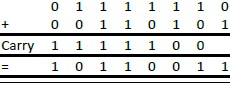
\includegraphics[width=0.3\textwidth]{pics/addition1.jpg}
		\columnbreak
		
		\subsubsection{Festkommazahlen}
			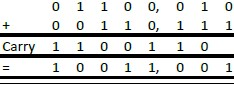
\includegraphics[width=0.3\textwidth]{pics/addition2.jpg}
		\columnbreak
		
		\subsubsection{Vorzeichen-Darstellung}
			\begin{minipage}[c]{1.5 cm}
				Es gilt: 
				\newline
			\end{minipage}
			\begin{minipage}[c]{3.5 cm}
				\begin{compactitem}
					\item 0$\rightarrow$positiv
					\item 1$\rightarrow$negativ
				\end{compactitem}
			\end{minipage}
			Beispiel:\\
			\begin{tabular}{llll}
				$+$ & 12310 & = & 0 111 1011\\
				$-$ & 12310 & = & 1 111 1011\\
			\end{tabular}
	\end{multicols}

\begin{multicols}{2}
	\subsection{Einerkomplement}
		Das Einerkomplement wird durch Invertieren aller Bits der positiven Zahl gebildet.\\
		$A_{k1}=\overline{A}$\\
		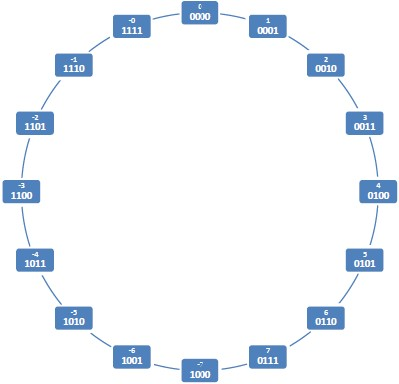
\includegraphics[width=0.4\textwidth]{pics/einerkomplement.jpg}	
		\columnbreak
		
	\subsection{Zweierkomplement}
		Das Zweierkomplement wird durch Invertieren aller Bits der positiven Zahl und der Addition von 1 gebildet.\\
		$A_{k2}=\overline{A}+1=(2^n-A)$\\
		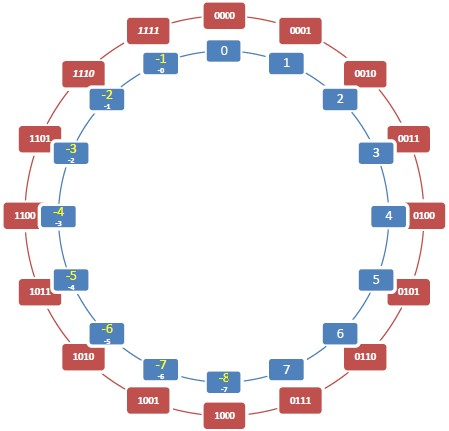
\includegraphics[width=0.4\textwidth]{pics/zweierkomplement.jpg}
\end{multicols}

\subsection{Subtraktion}
	F�r die Subtraktion A$-$B=C sind folgende Schritte notwendig:
	\begin{compactitem}
		\item 1) Der Subtrahend B muss ins Zweierkomplement gebracht werden.
		\item 2) Die arithmetische Operation muss durchgef�hrt werden.
		\item 3) Das Resultat muss korrekt interpretiert werden.
	\end{compactitem}
	In der Praxis bedeutet die Subtraktion von $2^n$, dass das Bit, welches an h�chster Stelle ($n+1$) steht, ignoriert wird.

\subsection{Bereichs�berschreitung}
	Bei Hardware ist die Wortbreite immer begrenzt, so kann es passieren, dass diese Wortbreite bei einer arithmetischen Operation �berschritten wird.\\
	Mit diesem Verfahren kann gepr�ft werden, ob eine Ergebnis korrekt ist:\\
	\ \newline
	\begin{tabular}{|l|l|l|}
		\hline
			Operation & Richtiges Ergebnis & �berlauf \\
		\hline
		\hline
			A$+$B & c$_n=0$, c$_{n-1}=0$ & c$_n=0$, c$_{n-1}=1$ \\
			A$-$B & c$_n=$c$_{n-1}$ & Nicht m�glich \\
			$-$A$-$B & c$_n=1$, c$_{n-1}=1$ & c$_n=1$, c$_{n-1}=0$ \\
		\hline		
	\end{tabular}
	
\subsection{Codes}
	\begin{minipage}[c]{5 cm}
		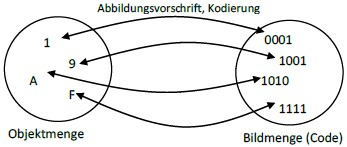
\includegraphics[width=0.9\textwidth]{pics/codes.jpg}
	\end{minipage}
	\begin{minipage}[c]{13 cm}
		Folgende Codes werden am h�ufigsten gebraucht:
		\begin{compactitem}
			\item Bin�rcode
			\item 
				\begin{tabbing}
					xxxxxxxxxxxxxxx\=xxxxxxxxxxxxxxxxxxxxxxxxxxxxxxxx\kill	
					Reiner Dualcode: \> Zuordnung von Dezimalzahlen den Bitfolgen des Dualsystems
				\end{tabbing}
			\item 
				\begin{tabbing}
					xxxxxxxxxxxxxxx\=xxxxxxxxxxxxxxxxxxxxxxxxxxxxxxxx\kill
					BCD Code: \> 
								\begin{tabular}{|lllllll|}
									\hline
										Dezimal & 1 & 2 & 3 & $\dots$ & 9 & \textgreater 9 \\
										BCD & 0001 & 0010 & 0011 & $\dots$ & 1001 & ung�ltig\\
									\hline
								\end{tabular}
				\end{tabbing}
		\end{compactitem}
	\end{minipage}